%!TEX root = draft.tex

% datasets table..
\begin{table*}[b]
 {
  \begin{tabular}[c]{llrrrc|rrrr} \toprule
   Network &  Description & $|V|$           & $|E|$        & $T$        & $A$, $|A|$  &  \texttt{LN} $(\mu, \sigma)$ & \texttt{DPL} $\alpha$       &  Avg. ${\texttt{LCC}}$  & \texttt{AA} $r$           \\ \midrule
   \texttt{USSC}~\cite{fowler2008authority}  & U.S. Supreme Court cases         & 30,288     & 216,738      & 1754-2002  & -   & (1.19, 1.18) & 2.32     & 0.12    & -     \\
   \texttt{HEP-PH}~\cite{gehrke2003overview} & ArXiv Physics manuscripts     & 34,546     & 421,533      & 1992-2002  & -  &   (1.32, 1.41) & 1.67     & 0.12    & -                 \\
   \texttt{Semantic}~\cite{ammar}&   Academic Search Engine  & 7,706,506  & 59,079,055   & 1991-2016  & -   &   (1.78, 0.96)  & 1.58     & 0.06    & -             \\   \midrule
   \texttt{ACL}~\cite{acldata}    & NLP papers      & 18,665     & 115,311      & 1965-2016  & \textsc{venue}, 50  &   (1.93, 1.38)  & 1.43     & 0.07    & 0.07  \\
   \texttt{APS}~\cite{aps}     & Physics journals     & 577,046    & 6,967,873    & 1893-2015  & \textsc{journal}, 13 &   (1.62, 1.20)  & 1.26     & 0.11    & 0.44 \\
   \texttt{Patents}~\cite{leskovec2005graphs}   & U.S. NBER patents    & 3,923,922  & 16,522,438   & 1975-1999  & \textsc{category}, 6 &   (1.10, 1.01)   & 1.94     & 0.04    & 0.72 \\
   % \texttt{PYPI}         & 25,169     & 71,371       & 2002-2018  & \textsc{category} & 9  \\
  \bottomrule
  \end{tabular}
  \vspace{1mm}
  \caption{Summary statistics \& global properties of six network datasets: $|V|$ nodes join the networks and form edges $|E|$ over
  time period $T$. In attributed networks, each node has a categorical attribute value that belongs to set $A$ of size $|A|$.
  The networks exhibit lognormal (\texttt{LN}) in-degree distribution with mean $\mu$ and standard deviation $\sigma$,
  high average local clustering (${\texttt{LCC}}$) \& attribute assortativity (\texttt{AA}) coefficient and
  densify over time with power law (\texttt{DPL}) exponent $\alpha$.}
  \label{table:datasets}
  \label{table:netstats}
 }
\end{table*}


\section{Introduction}
\label{sec:Introduction}


% what is the problem?

In this paper, we present a network growth model that explains how distinct
structural properties of attributed networks can emerge from local edge
formation processes. In real-world networks, individuals tend to form edges
under resource constraints such as limited information and partial network
access. Additionally, sociological phenomena such as triadic closure and
homophily \textit{simultaneously} impact individuals’ decisions to form edges.
Over time, these decisions cumulatively shape real-world networks as they
exhibit rich structural characteristics: heavy-tailed indegree distribution,
skewed local clustering and homophilic mixing patterns. However, we lack
mechanisms that incorporate the effect of resource constraints and
\textit{multiple} sociological factors on edge formation as well as preserve
global network structure.

% why is it important?

Existing models of network growth tend to make unrealistic assumptions about how
individuals form edges. Consider a simple stylized example: the process of
finding a set of papers to cite when writing an article. In preferential
attachment \cite{barabasi1999emergence} or fitness \cite{X} based models, a node
making $m$ citations would pick papers from the \textit{entire} network in
proportion to their indegree or fitness respectively. This process assumes that
individuals possess complete knowledge of indegree or fitness of every node in
the network. An equivalent formulation — vertex copying \cite{X} — induces
preferential attachment: for every citation, a node would pick a paper uniformly
at random from \textit{all} papers, and either cite it or copy its citations.
Notice that the copying mechanism assumes individuals have complete access to
the network and form each edge independently. Although these models explain the
emergence of power law degree distributions, they are unrealistic
representations of how individuals make decisions about edge formation. A
realistic representation of how individuals form edges necessitates modeling the
effect of multiple sociological phenomena on edge formation under resource
constraints.

%why is it hard?
The problem of developing a model of network growth, where individuals act under
resource constraints, including access to only local information is hard. The
problem lies in identifying simple mechanisms with few parameters that unifies
multiple sociological phenomena to \textit{jointly} preserve structural
properties and attribute mixing patterns of attributed networks.

% what did we do?


We propose an Attributed Random Walk \texttt{ARW} model that jointly explains
the emergence of in-degree distributions, local clustering, clustering-degree
relationship and attribute mixing patterns through a resource constrained mechanism
based on random walks.
In \texttt{ARW}, incoming nodes select a seed node based on attribute similarity
and initiate a biased random walk: At each step of the walk, the incoming node either
jumps back to its seed or chooses an outgoing link or incoming link to visit another
node. It links to each visited node with some probability and halts after forming a
few connections. We have three primary contributions:
\begin{itemize}
\item model effect of multiple sociological phenomena on edge formation simulatenously
\item provide a realistic representation of how individuals form edges under constraints of limited information and partial network access.
\item jointly preserve key structural properties and attribute mixing patterns of real-world attributed networks.
\end{itemize}

\begin{figure}[t]
 \centering
 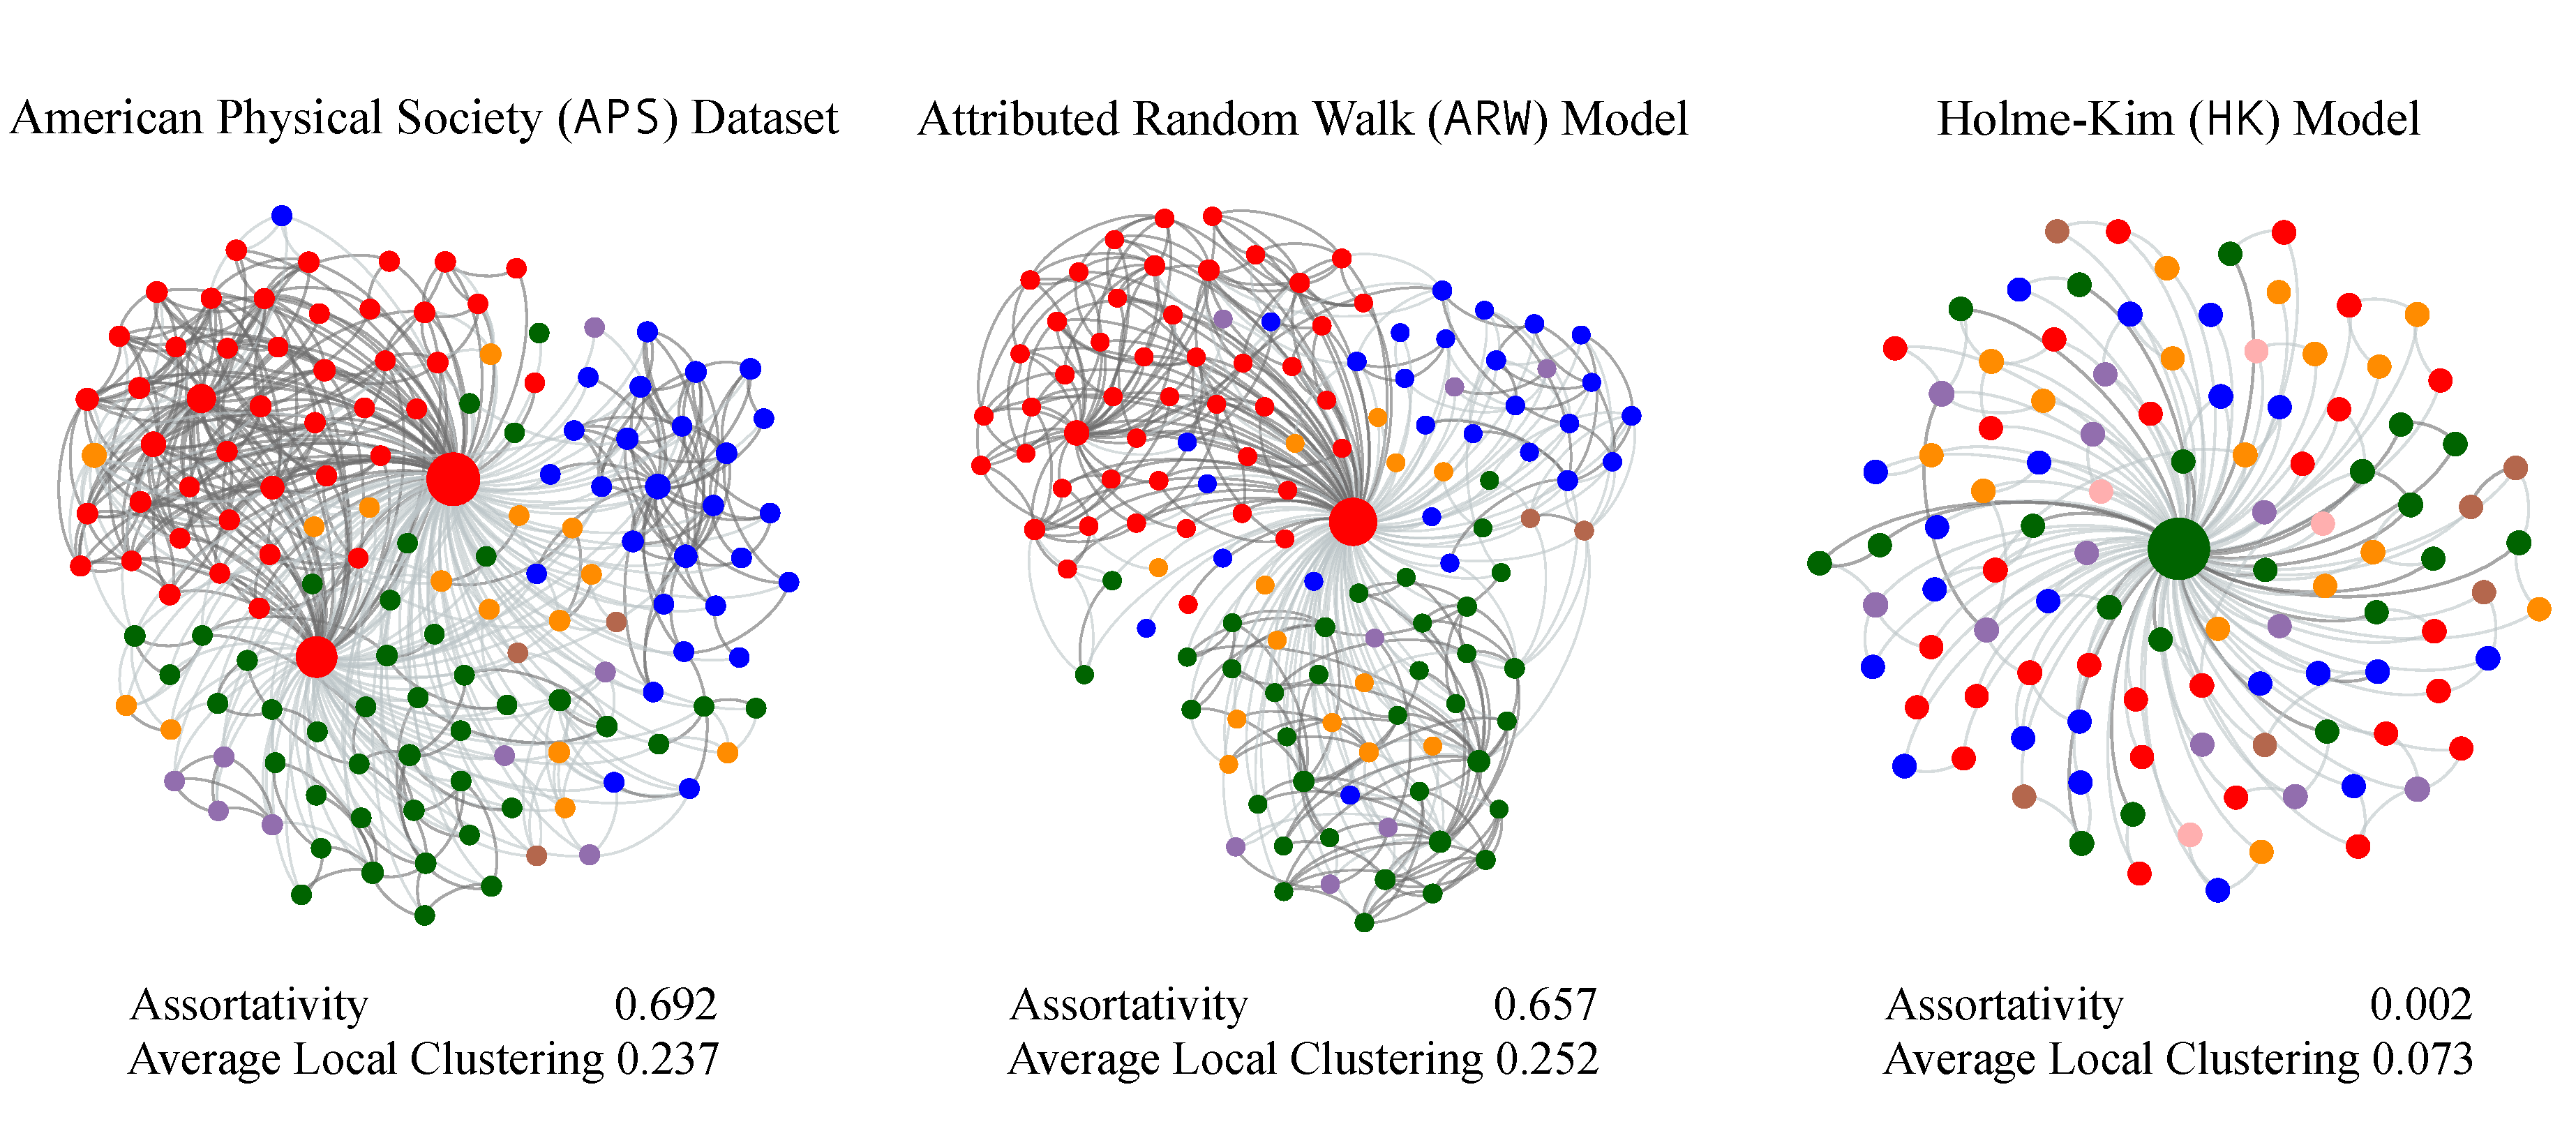
\includegraphics[width=\columnwidth]{experiments_final4}
 \caption{
 }
 \label{fig:intro_plot}
\end{figure}

We conducted extensive experimental results, against state of the art
baselines, on large citation network datasets. We show that our growth model
outperforms that best competing model in jointly and accurately preserving
multiple structural properties---degree distribution, clustering and
degree-clustering relationship---by a significant margin.

The rest of the paper is organized as follows.
We begin by defining the problem statement in~\Cref{sec:Problem Statement}.
In~\Cref{sec:Analysis}, we outline six network datasets, describe key structural
properties of real-world networks and discuss insights from sociological studies.
Then, in~\Cref{sec:Proposed Model}, we describe the network growth model. This
is followed by experiments in~\Cref{sec:Experiments} \&~\Cref{subsec:LocalMixing}
and discussion in~\Cref{sec:Discussion}.

% In~\Cref{sec:Related Work}, we
% describe the related work. Then, in~\Cref{sec:Preliminaries}, we define key
% structural properties and introduce the datasets. We formally state the goal of
% the paper in~\Cref{sec:Problem Statement}. In~\Cref{sec:Empirical Analysis}
% and~\Cref{sec:Proposed Model}, we report prominent structural characteristics
% of citation networks and propose a network growth model respectively. This is
% followed by~\Cref{sec:Experiments}, where we validate our model against
% multiple baselines.